



\iffalse
Las relaciones de equivalencia en un conjunto sirven fundamentalmente para
obtener clasificaciones de los elementos del conjunto. Estas clasificaciones
se hacen mediante las clases de cquivalencia. La idcntifieación de todos los
conjuntos de una clase de equivalencia conduce al concepto de conjunto
cociente. Este concepto es de gran utilidad para definir nuevos conjuntos
partiendo de uno determinado, como haremos en los ejemplos TKTK y TKTK.
\fi

Definición. Relación de equivalencia. Una relación $\erel$ en el conjunto
$U$ se denomina \semph{relación de equivalencia} cuando posee las
propiedades reflexiva, simétrica y transitiva.

\begin{example}
  Relación de equipolencia entre vectores. En el conjunto de vectores fijos
  del plano o del espacio, la relación de equipolencia es un relación de
  equivalencia. Recuérdese que un vector fijo es un segmento orientado (o
  dirigido) y que está compuesto por un punto origen del segmento, una recta
  dirección sobre la que se dibuja el segmento, la longitud del segmento y
  el sentido. El vector $\vec{v}$ es equipolente al vector $\vec{w}$ si y
  solo si las rectas directrices son la misma o paralelas y los módulos y
  sentidos son iguales.

  Además, cada uno de los conjuntos constituidos por todos los vectores que
  son equipolentes entre sí es denominado \emph{vector libre}.

  A la vista de este ejemplo, podemos ver que hemos hecho una clasificación
  de los vectores. Vamos a hablar ahora sobre esto mismo de forma más
  general.
\end{example}

Definición. Clase de equivalencia. Dada una relación de equivalencia $\erel$
en un conjunto $U$, se denomina \semph{clase de equivalencia} del elemento
$x \in U$ al conjunto imagen de $x$, que denotamos $x\erel$ o $[x]$, es
decir,

\[ [x] = \{y \in U \st x \erel y, \ x \in U\} \]

Muchas veces, se habla simplemente de \emph{clase}, cuando se sobrentiende
que nos referimos a clases de equivalencia.




\subsection{Propiedades}

Dada una relación de equivalencia homogénea $\erel \subseteq U \times U$ y
tres elementos $x, y, z \in U$, se cumple

\begin{proposition}
  1. Propiedad. Si $x \erel y$, entonces $[x] = [y]$.
\end{proposition}

\begin{proof}
  Se puede demostrar deduciéndolo de forma directa de los requisitos en la
  definición de relación de equivalencia.

  Para cada $z \in [x]$, se tiene que $x \erel z$ y, ya que en toda relación
  de equivalencia se debe cumplir la propiedad simétrica, también se cumple
  $z \erel x$. Dado que $z \erel x$ y $x \erel y$, se tiene entonces, por la
  propiedad transitiva, que $z \erel y$. Aplicando otra vez la propiedad
  simétrica, se tendrá que $y \erel z$, que es lo mismo que decir que $z \in
  [y]$. Con esto hemos llegado a demostrar que $[x] \subseteq [y]$. De forma
  análoga se comprueba que $[y] \subseteq [x]$. Ambas afirmaciones hacen que
  se cumpla $[x] = [y]$.
\end{proof}

\begin{proposition}
  2. Propiedad. Si $x \not\erel y$, entonces $[x] \cap [y] = \emptyset$.
\end{proposition}

\begin{proof}
  Vamos a demostrarla por contradicción. Suponemos que $[x] \cap [y] \neq
  \emptyset$, que sería lo mismo que decir que existe un $z \in [x] \cap
  [y]$, o, lo que es lo mismo, se tiene que $x \erel z$ e $y \erel z$. Al
  aplicar, al igual que en la otra demostración, las propiedades simétrica y
  transitiva, se puede llegar a obtener que $x \erel y$, cosa que contradice
  la hipótesos $x \not \erel y$. Por tanto, se tiene que $[x] \cap [y] =
  \emptyset$.
\end{proof}

Muchas veces, al trabajar con clases de equivalencia, hacemos uso de un
elemento de una clase para hablar de todos. A este elemento al que se le da
esa utilidad se le denomina \semph{representante} de esa clase de
equivalencia.

\begin{example}
  Ecuaciones de la recta en el plano euclídeo. En el conjunto

  \[ E = \{ax + by + c = 0 \st |a| + |b| \neq 0, \ a, b, c \in \rset\} \]

  \noindent de las ecuaciones con coeficientes reales en dos incógnitas, se
  define la relación de equivalencia siguiente. Para $a, b, c, e, f, g \in
  \rset$,

  \[ (ax + by + c = 0) \erel (ex + fy + g = 0) \]

  \noindent si y solo si los coeficientes de las ecuaciones son
  proporcionales. Es decir, de forma simbólica,

  \[ \exists p \in \rset, \ p \neq 0, \ \text{tal que} \ a = pe, \ b = pf \
  \text{y} \ c = pg \]

  \noindent Por cierto, quizás, se pregunte por qué se ponen esos valores
  absolutos en la expresión del conjunto $E$, es decir, $|a| + |b| \neq 0$.
  La razón está en que deseamos excluir el caso de $a = b = 0$, para el que
  la gráfica no sería una recta sino un punto, pero preferimos expresarlo de
  un modo algo más ``elegante'', si se puede llamar ``elegante'' a eso.

  En esa relación, cada clase de equivalencia se corresponde con una recta
  en el plano euclídeo dotado de un sistema de referencia, es decir, si las
  ecuaciones tienen los coeficientes proporcionales, entonces esas
  ecuaciones representan la misma recta. De esta forma, a clases de
  equivalencia distintas le corresponden rectas distintas. A la hora de
  trabajar con una recta, se elige la ecuación representante de la clase de
  equivalencia que más interese. De esta forma, en lugar de trabajar con un
  elemento geométrico, se trabaja con un elemento algebraico.
\end{example}

\begin{example}
  Dirección en el plano euclídeo. Se supone que el plano euclídeo está
  dotado de un sistema de referencia. En el conjunto de rectas del plano se
  define una relación de equivalencia. Dos rectas $r$ y $r'$ son paraleleas,
  cosa que solemos designar por $r || r'$, si y solo si los coeficientes de
  las incógnitas de sus ecuaciones son proporcionales. Al emplear una
  ecuación de cada recta:

  \begin{align*}
    r   &\equiv ax + by + c = 0 \\
    r'  &\equiv ex + fy + g = 0 \\
  \end{align*}

  \noindent se tiene

  \[ r || r' \iff \exists p \in \rset, \ p \neq 0, \ \text{tal que} \ a = pe
  \ \text{y} \ b = pf \]

  A cada clase de equivalencia le corresponde lo que se llama una
  \emph{dirección} en el plano euclídeo, es decir, una dirección es el
  conjunto de una recta y todas sus paralelas.
\end{example}

\begin{example}
  Vector libre del plano euclídeo. Cada vector libre del plano o del espacio
  es una clase de equivalencia de la relación de equipolencia del ejemplo
  TKTK en el conjunto de los vectores fijos del plano o del espacio. Cuando
  se interpretan geométricamente resultados con vectores libres, se utilizan
  vectores fijos escogiendo representantes adecuados.
\end{example}

Definición. Conjunto cociente. Dada una relación de equivalencia $\erel
\subseteq U \times U$, se denomina \semph{conjunto cociente}, $U/\erel$, al
conjunto de todas las clases de equivalencia que se generan en esa relación
$\erel$.

\begin{example}
  Números enteros ($\zset$). En el conjunto de los números naturales,
  $\nset$, se puede plantear preguntas del estilo: ¿Qué número natural al
  sumarle 3 da como resultado 5? Es decir, se plantea la ecuación $x + 3 =
  5$, que tiene solución. Pero si se plantea la ecuación $x + 5 = 3$, ocurre
  que no existe solución en $\nset$.

  En general, una ecuación de la forma $x + b = a$, donde $a$ y $b$ son
  números naturales, no siempre posee solución en el conjunto $\nset$.
  Buscar un marco donde esta ecuación genérica posea solución es lo que
  obliga a introducir el conjunto de los números enteros, denotado por
  $\zset$.

  La ecuación $x + b = a$ tiene solución en $\nset$ dependiendo del par de
  números $(a, b)$. Esto nos induce a pensar en definir los números enteros
  partiendo de pares de números naturales. Además, los pares ($5, 3)$, $(8,
  6)$ y $(3, 1)$ inducen ecuaciones que tienen la misma solución, $x = 2$,
  esto lleva a considerar el conjunto $\nset \times \nset$ y la relación de
  equivalencia siguiente:

  \[ (a, b) \erel (c, d) \ \text{si y solo si} \ a + d = b + c \]

  \noindent Piense como si esto viniera de $a - b = c - d$, que al fin y al
  cabo es la misma ecuación, pero la definición debe hacerse con la suma, en
  lugar de la resta. TKTK.

  El conjunto cociente $(\nset \times \nset)/\erel$, denotado normalmente
  como $\zset$, está compuesto por las clases

  \[ [(0, 0)], [(1, 0)], [(0, 1)], [(2, 0)], [(0, 2)], \ldots \]

  \noindent que se designan también por $0, 1, {-1}, 2, {-2}, \ldots$ Así,
  pues, el conjunto $\zset$ se escribe

  \[ \zset = \{\ldots, {-3}, {-2}, {-1}, 0, 1, 2, 3, \ldots\} \]

  Observación. Al igual que en $\nset$, la notación $\zset^*$ designa a
  $\zset \setminus \{0\}$.
\end{example}

\begin{example}
  Números racionales ($\qset$). En el conjunto de los números enteros,
  $\zset$, se pueden plantear preguntas del estilo: ¿Qué número entero
  multiplicado por 2 da como resultado 6? Es decir, se plantea la ecuación
  $2x = 6$, que tiene solución. Pero si se plantea la ecuación $6x = 2$,
  ocurre que no existe solución en $\zset$.

  En general, una ecuación de la forma $bx = a$, donde $b \neq 0$ y $a$ son
  números enteros, no siempre tiene solución en el conjunto $\zset$. Buscar
  un marco donde esta ecuación genérica tenga solución es lo que obliga a
  introducir el conjunto de los números racionales, denotado $\qset$.

  La ecuación $bx = a$ tiene solución en $\zset$ dependiendo del par de
  números $(a, b)$. lo que nos induce a pensar en definir los números
  racionales partiendo de pares de números enteros, teniendo en cuenta que
  el $b$ no puede valer 0. Además, observamos que los pares $(3, 1)$, $(6,
  2)$ y $(15, 5)$ conducen a la misma solución de la correspondiente
  ecuación. Esto nos lleva a considerar en el conjunto $\zset \times
  \zset^*$ la siguiente relación de equivalencia:

  \[ (a, b) \erel (c, d) \ \text{si y solo si} \ ad = bc \]

  \noindent Piense como si esto viniera de $a/b = c/d$, que al fin y al cabo
  es la misma ecuación, pero la definición debe hacerse con el producto, en
  lugar de la división. TKTK.

  El conjunto cociente $(\zset \times \zset^*)/\erel$, que denotamos por
  $\qset$, se escribe como

  \[ \frac{a}{b} \]

  \noindent Así, pues, el conjunto $\qset$ se escribe como

  \[ \qset = \left\{ \frac{a}{b} \st \right. (a, b) \in \zset \times
  \zset^*\} \]

  Al igual que con $\zset$, la notación $\qset^*$ designa a $\qset \setminus
  \{0\}$.
\end{example}

\begin{example}
  Enteros módulo $p$: $\zset/p$. En el conjunto de los números enteros,
  $\zset$, se define la relación de equivalencia

  \[ a \equiv b \pmod p \ \text{si y solo si} \ a - b \ \text{es divisible
  por} \ p \]

  \noindent o, dicho de otro modo,

  \[ a \equiv b \pmod p \iff \exists k \in \zset. \ a - b = kp \]

  \noindent Esto también se puede decir como que los restos de la división
  entera de $a$ y $b$ entre $p$ coinciden. Esta relación $a \equiv b \pmod
  p$ se lee como ``$a$ es congruente con $b$ módulo $p$''.

  El conjunto cociente $\zset/\equiv$, que denotamos por alguna de las
  expresiones siguientes: $\zset/p\zset$, $\zset/(p)$ o $\zset/p$, está
  compuesto por las clases $[0], [1], [2], [3], \ldots, [p-1]$, que
  denominamos simplemente

  \[ \zset/p = \{0, 1, 2, 3, \ldots , (p-1)\} \]

  Si se fija, la clase del $0$, es decir, $[0]$, sería el conjunto de todos
  los múltiplos de $p$, es decir,

  \[ p\zset = \{kp \st k \in \zset\} \]
\end{example}

\begin{example}
  Números reales módulo $2\pi$: $\rset/2\pi$. En el conjunto de los números
  reales, $\rset$, se define la relación de equivalencia

  \[ a \equiv b \pmod {2\pi} \ \text{si y solo si} \ \exists k \in \zset \
  \text{tal que} \ a - b = 2\pi k \]

  \noindent o, lo que es lo mismo,

  \[ a \equiv b \pmod {2\pi} \iff \exists k \in \zset, \ a = b + 2\pi k \]

  El conjunto cociente $\rset/\equiv$, que denotamos por alguna de las
  expresiones siguientes: $\rset/2\pi\zset$, $\rset/(2\pi)$ o $\rset/2\pi$,
  está compuesto por las clases $[r]$ donde $r \in [0, 2\pi)$. Las medidas
  de los ángulos en radianes son una buena interpretación de este conjunto
  cociente. Las funciones priódicas de periodo $2\pi$ tan solo se estudian
  en el intervalo $[0, 2\pi]$, o en el $[{-\pi}, \pi]$, puesto que la
  gráfica en el intervalo $[(2k - 1)\pi, [(2k + 1)\pi]$ es la misma que en
  el intervalo $[{-\pi}, \pi]$.
\end{example}

Definición. Partición de un conjunto. Una \semph{partición} de un conjunto
$U$ es una familia $P$ de subconjuntos no vacíos de $U$ disjuntos dos a dos
y cuya unión es el conjunto $U$.

Se podría dar una definición alternativa, más simbólica.

Una partición de un conjunto $U$ es un conjunto de $n \in \nset$ conjuntos
$A_1, A_2, A_3, \ldots, A_n$ no vacíos para los que, para todos los índices
$i, j \in \nset$, siendo $1 \leq i \leq n$, $1 \leq j \leq n$ e $i \neq j$,
se cumplen

\begin{center}
  \begin{tabular}{lr}
    $\bigcup_{A_i \subseteq U} A_i = U \quad$ y
      & $\quad A_i \cap A_j = \emptyset$ \\
  \end{tabular}
\end{center}

De esta definición, se derivan algunos hechos importantes.

Toda relación de equivalencia $\erel \subseteq U \times U$ genera una
partición de $U$ puesto que, tal y como demostramos antes, las clases
$U/\erel$ son subconjuntos de $U$ disjuntos dos a dos y, por definición, la
unión de estos es el conjunto $U$.

Recíprocamente, toda partición $P$ del conjunto $U$ permite definir la
siguiente relación de equivalencia $\erel$ en el conjunto $U$:

$$ x \erel y \ \text{si y solo si existe algún} \ A \in P \ \text{tal que} \
\{x, y\} \subseteq A $$

% TODO Esto se puede demostrar, y no es fácil hacerlo. Se hace en el libro
% de Newstead.

\begin{example}
  Gráficas de superficies por ordenador. Al intentar representar una
  superficie definida por una ecuación en un ordenador, por ejemplo el
  paraboloide $z = x^2 +3y^2$, se debe determinar el dominio en el que se
  dibujará. Generalmente, se trata de un dominio rectangular, por ejemplo
  $[0, 1] \times [0, 1]$. El programa con opciones gráficas establece una
  partición del dominio en cuadradillos de lados paralelos a los lados del
  dominio rectangular, a modo de rejilla rectangular. Entonces, el programa
  establece su \emph{grid} (rejilla) o nube de puntos del dominio, que sude
  ser algún vértice de cada cuadradillo $(x_i, y_i)$, para proceder al
  cálculo de los valores $z_i$ correspondientes, y construye la nube de
  puntos del espacio $(x_i, y_i, z_i)$. Esencialmente, este proceso
  establece el conjunto cociente correspondiente a la relación definida por
  la partición del dominio, y se elige un representante de cada clase para
  valorar la altura de la superficie en esos representantes, en general, un
  vértice del cuadradillo. Es decir, se pasa de un dominio continuo a un
  dominio discreto de clases y se considera la altura de cualquier elemento
  de una clase como la altura del elemento seleccionado de esa clase. La
  construcción ``continua'' que muestran los ordenadores es una cuestión que
  no abordamos. Vea las figuras~\ref{fig:rejilla-superficie}
  y~\ref{fig:nube-puntos-superficie}.

  \begin{figure}
    \centering
    \foreignlanguage{english}{
    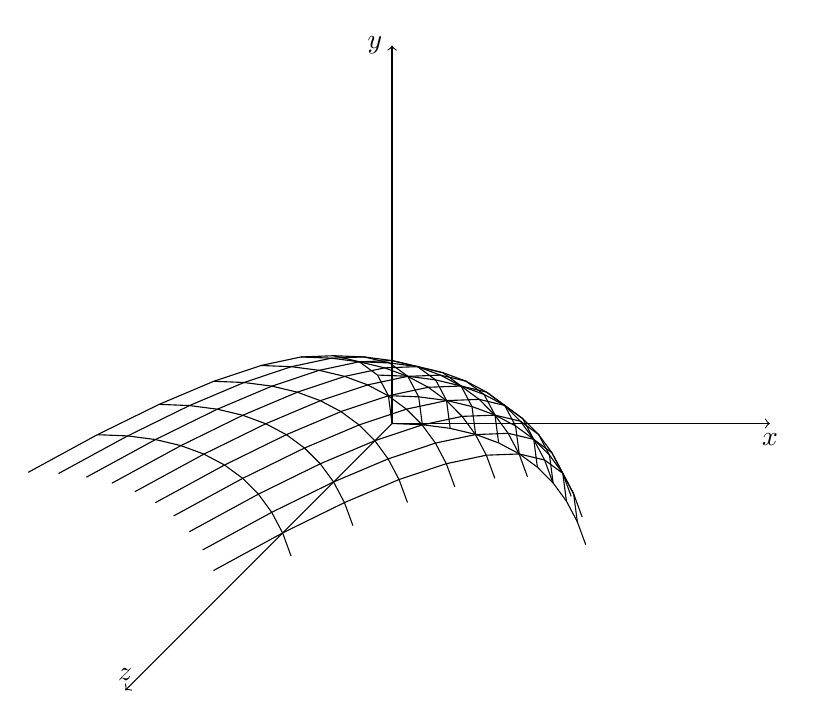
\begin{tikzpicture}[scale=4]

      % Dibujar los ejes
      \draw[->] (0,0,0) -- (1.2,0,0) node[below] {$x$};
      \draw[->] (0,0,0) -- (0,1.2,0) node[left] {$y$};
      \draw[->] (0,0,0) -- (0,0,2.2) node[above] {$z$};

      % Parámetros
      \def\xmin{0} % Inicio del rango en x
      \def\xmax{1} % Fin del rango en x
      \def\ymin{0} % Inicio del rango en y
      \def\ymax{1} % Fin del rango en y
      \def\step{0.1} % Tamaño del paso

      % Dibujar la rejilla de la superficie
      \foreach \x in {\xmin,\step,...,\xmax} { % Iterar sobre x
        \foreach \y in {\ymin,\step,...,\ymax} { % Iterar sobre y
          \pgfmathsetmacro{\z}{\x*\x + 3*\y*\y} % Calcular z = x^2 + 3y^2
          % z para (x+step)
          \pgfmathsetmacro{\znextx}{(\x+\step)*(\x+\step) + 3*\y*\y}
          % z para (y+step)
          \pgfmathsetmacro{\znexty}{\x*\x + 3*(\y+\step)*(\y+\step)}


          % Dibujar líneas en la dirección de x
          \ifdim \x pt<\xmax pt
            \draw[thin] (\x,\y,\z) -- ({\x+\step},\y,\znextx);
          \fi

          % Dibujar líneas en la dirección de y
          \ifdim \y pt<\ymax pt
            \draw[thin] (\x,\y,\z) -- (\x,{\y+\step},\znexty);
          \fi
        }
      }

    \end{tikzpicture}
    }
    \caption{Rejilla de la superficie $z = x^2 + 3y^2$.}%
    \label{fig:rejilla-superficie}
  \end{figure}

  \begin{figure}
    \centering
    \foreignlanguage{english}{
    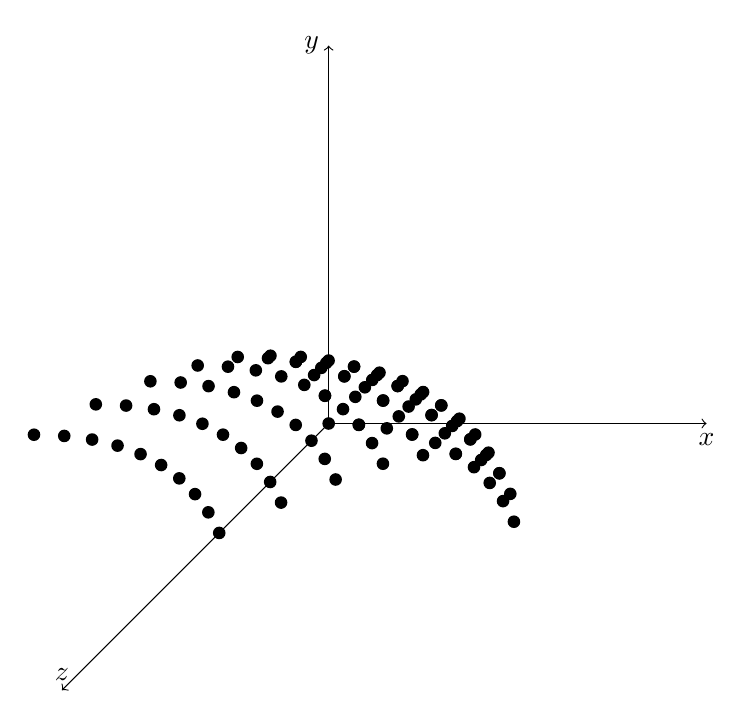
\begin{tikzpicture}[scale=4]

      % Dibujar los ejes
      \draw[->] (0,0,0) -- (1.2,0,0) node[below] {$x$};
      \draw[->] (0,0,0) -- (0,1.2,0) node[left] {$y$};
      \draw[->] (0,0,0) -- (0,0,2.2) node[above] {$z$};

      % Parámetros
      \def\xmin{0} % Inicio del rango en x
      \def\xmax{1} % Fin del rango en x
      \def\ymin{0} % Inicio del rango en y
      \def\ymax{1} % Fin del rango en y
      \def\step{0.1} % Tamaño del paso

      % Dibujar la nube de puntos de la superficie
      \foreach \x in {\xmin,\step,...,\xmax} { % Iterar sobre x
        \foreach \y in {\ymin,\step,...,\ymax} { % Iterar sobre y
          \pgfmathsetmacro{\z}{\x*\x + 3*\y*\y} % Calcular z = x^2 + 3y^2
          \fill (\x,\y,\z) circle[radius=0.02]; % Dibujar punto
        }
      }

    \end{tikzpicture}
    }
    \caption{Nube de puntos de la superficie $z = x^2 + 3y^2$.}%
    \label{fig:nube-puntos-superficie}
  \end{figure}
\end{example}

\begin{example}
  Al considerar la partición

  \[ P = \{[i - 1, i) \st i \in \zset\} \]

  \noindent de intervalos en $\rset$, se define la relación de equivalencia
  entre números reales $x \rrel y$ si y solo si existe un intervalo $[i-1,
  i)$ tal que $x, y \in [i-1, i)$. Es decir, dos números reales están
  relacionados si y solo si tienen la misma parte entera.
\end{example}





